\section{Making a Monte Carlo integrator}
\label{ch:monte_app}

First, we explored different methods in order to gain a better insight on how to create a good general integrator. We tested 4 methods, where each differs in how the points in the domain are chosen to evaluate the integral (compare to chapter~\ref{ch:monte}):
\begin{enumerate}
  \item Uniform Static - The entire domain is divided by a uniform mesh were each point is taken in a coordinate is the grid.
  \item Uniform Adaptive - The domain is divided uniformly in square boxes, and for each box a mesh grid is created
  specified by a density value which determines the total number of points inside that box. The density parameter
  is obtained by performing successive iterations, on which the density of each sub-box is set by the total value of the integral inside
  the box.
  \item Stratified Static - The entire domain is divided in a uniform mesh, where for each quadrant of the mesh
  a single point is chosen randomly inside.
  \item Stratified Adaptive - A combination of both methods adaptive and stratified.
\end{enumerate}
\begin{figure*}
  \begin{center}
    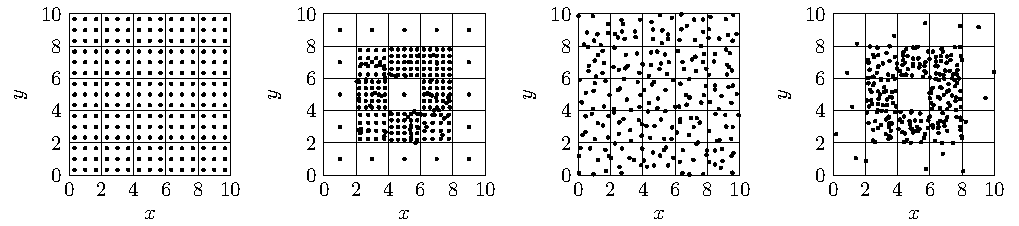
\includegraphics[scale=1 ]{graphs/BoxPlotter.pdf}
  \caption{Illustrative examples of (from left to right) a uniform static, uniform adaptive, stratified static and stratified adaptive integration schemes. The lines create boxes within which an internal grid is applied in the case of static integration schemes. Notice that in all cases the number of points is the same, which in the case of adaptive static causes us to end with some points which do not fit in a grid. To accommodate for this we distributed them randomly within their respective box. }
\label{BoxPlotter}
  \end{center}
\end{figure*}

To compare these methods we used a ring-shaped test function over which we evaluated the integrals. This two-dimensional ring, with an outer radius of 4 and an inner radius of 2, the value is 2, outside it is zero. The analytical integral over the whole domain is thus simply $ A=2\pi (4^2-2^2)$.  In figure~\ref{BoxPlotter} a set of sampling point distributions for this test function and each method are shown. To compare the performance of these methods, each of them were executed at a different number of test points. The obtained results were compared with the analytical answer and over several repetitions the average error determined. These results are shown in fig. \ref{MCerrs}, where 1,000 repetitions where used for each number of points. In the case of adaptive methods the entire integration domain was divided into 25 boxes.

One can clearly see, that only certain number of points can be achieved with the uniform methods, since the points always need to fit in a grid. For the uniform static method no deviation can be seen. This is due to the fact, that this method is fully deterministic and thus all repetitions with the same parameters return the same result.
As expected the best results are obtained with the adaptive stratified method, which has also gives the smallest standard deviation from the error as seen in the error bars (with the exception of the uniform static method).
Additionally it is important to note how the error of the uniform static method, and in lesser degree in the adaptive static, increases at some point as the number of points increases, this systematic error introduced by the regular mesh. This shows the entire point of doing Monte Carlo integration!
\begin{figure*}[ht]
  \begin{center}
  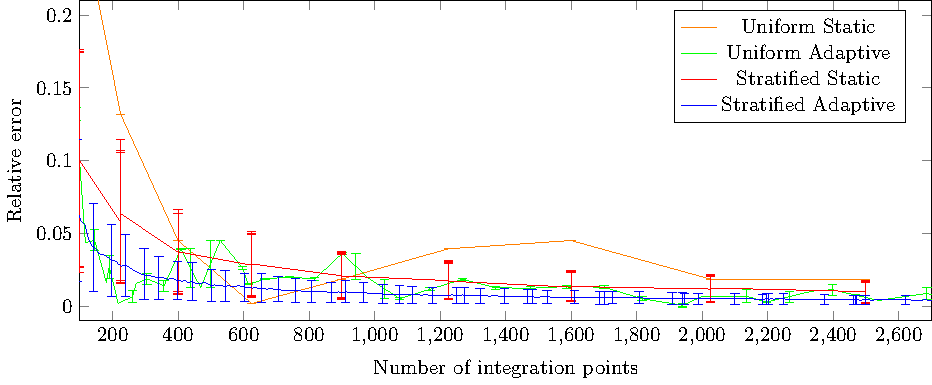
\includegraphics[scale=1 ]{graphs/integration_test_ring.pdf}
  %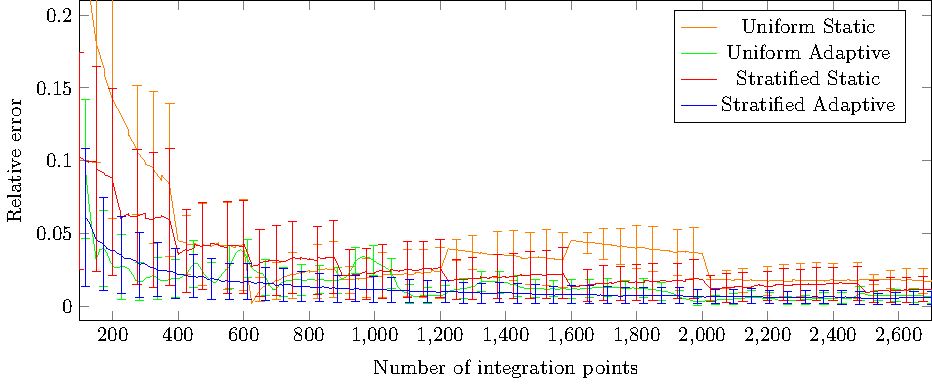
\includegraphics[scale=1 ]{graphs/integration_test_ring_rand.pdf}
  \caption{Performance comparison of different numeric integration methods. The absolute value of the difference between the numerically calculated result and the analytical answer plotted against the number of integration points used. The used function is a two-dimensional ring (see text).}
  \label{MCerrs}
  \end{center}
\end{figure*}
